\section[Introdução]{Introdução}

O \textbf{Amores Fati} é um projeto desenvolvido para o \textbf{Instituto Amores Fati},
organização do terceiro setor que atua na inclusão de pessoas com deficiência (\ac{pcd}) e
jovens em situação de vulnerabilidade social no mercado de trabalho digital, por meio do
programa de cursos gratuitos \textit{FATLAB}. A iniciativa foi inspirada na trajetória de
Pedro Felipe Rosinha, que, superando suas dificuldades, conseguiu se inserir no mercado
de tecnologia e construir uma carreira sólida.

O instituto conta com apoio da \ac{pucrs} e tem sua central de atendimento instalada dentro
do Parque Tecnológico TECNOPUC. Com recursos provenientes exclusivamente de doações, surgiu
a necessidade de um sistema desenvolvido pela \ac{ages} para gerenciar os processos internos
e gerar indicadores que auxiliem na captação de novos apoiadores.

\textbf{Stakeholders:} Martha Rosinha e Pedro Felipe Rosinha (Instituto Amores Fati).

\textbf{Período de Execução:} 2026/1 --- 2ª-feira e 4ª-feira, das 17h30 às 19h00.

\begin{figure}[H]
    \centering
    \small
    \caption{Time Amores Fati}
    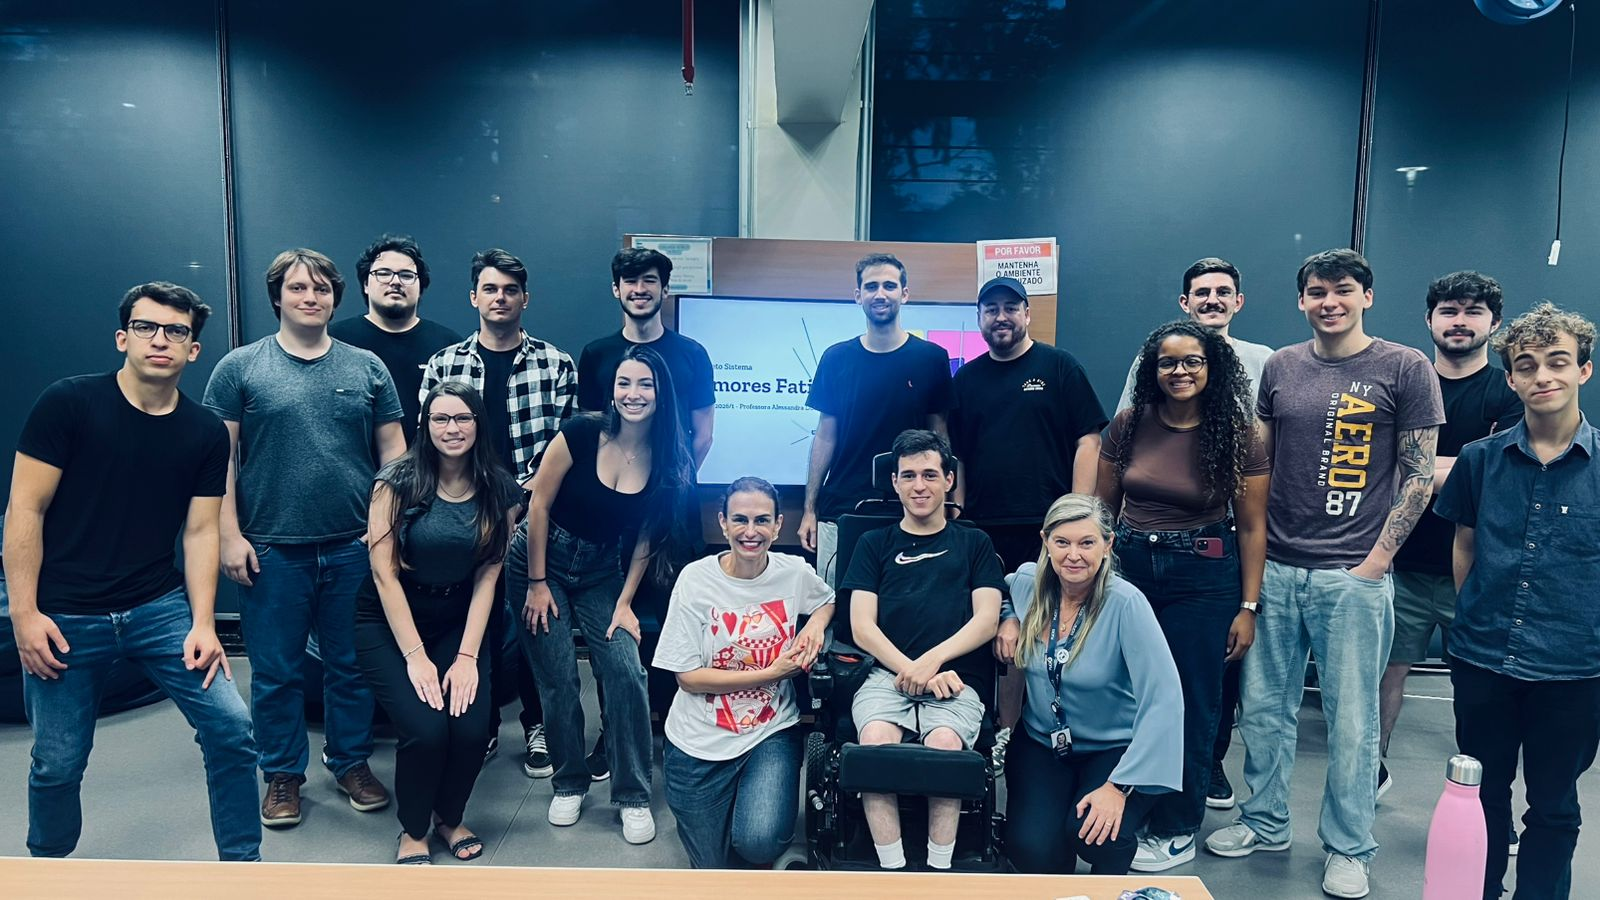
\includegraphics[width=1\linewidth]{conteudo//3 - ages II//conteudo//figures/TimeAF.png}
    Fonte: Arquivos pessoais
    \label{fig:time-amores-fati}
\end{figure}
